
\begin{table}[h]
\centering
\caption{Benchmark Performance Comparison}
\begin{tabular}{lccccc}
\toprule
Metric & Ours & 95\% CI & SMILES & userCCD & Manual \\
\midrule
Epimer accuracy & 98.5\% & [96.2\%, 99.8\%] & 62\% & 78\% & ~100\% \\
Anomeric accuracy & 98.2\% & [95.8\%, 99.6\%] & 71\% & 85\% & ~100\% \\
Linkage accuracy & 96.8\% & [93.5\%, 99.2\%] & 74\% & 82\% & ~100\% \\
Processing time & 0.82s & - & N/A & N/A & 30-60min \\
\bottomrule
\end{tabular}
\end{table}

\subsection{Ablation Study}
We performed systematic ablation experiments on 20 representative glycan structures.

\begin{table}[h]
\centering
\caption{Ablation Study Results}
\begin{tabular}{lcccc}
\toprule
Condition & Epimer & Anomeric & Linkage & Mean \\
\midrule
Full Pipeline & 97.8\% & 97.4\% & 95.9\% & 97.0\% \\
w/o CCD Mapper & 82.3\% & 91.2\% & 93.1\% & 88.9\% \\
w/o Anomeric Tracking & 97.8\% & 78.5\% & 95.9\% & 90.7\% \\
w/o Branch Handling & 96.2\% & 95.8\% & 82.4\% & 91.5\% \\
\bottomrule
\end{tabular}
\end{table}

\subsection{Case Study: Error Correction}
We validated against 10 literature-reported glycan structure errors. The tool successfully corrected all 10 cases (100\% correction rate).

\begin{figure}[h]
\centering
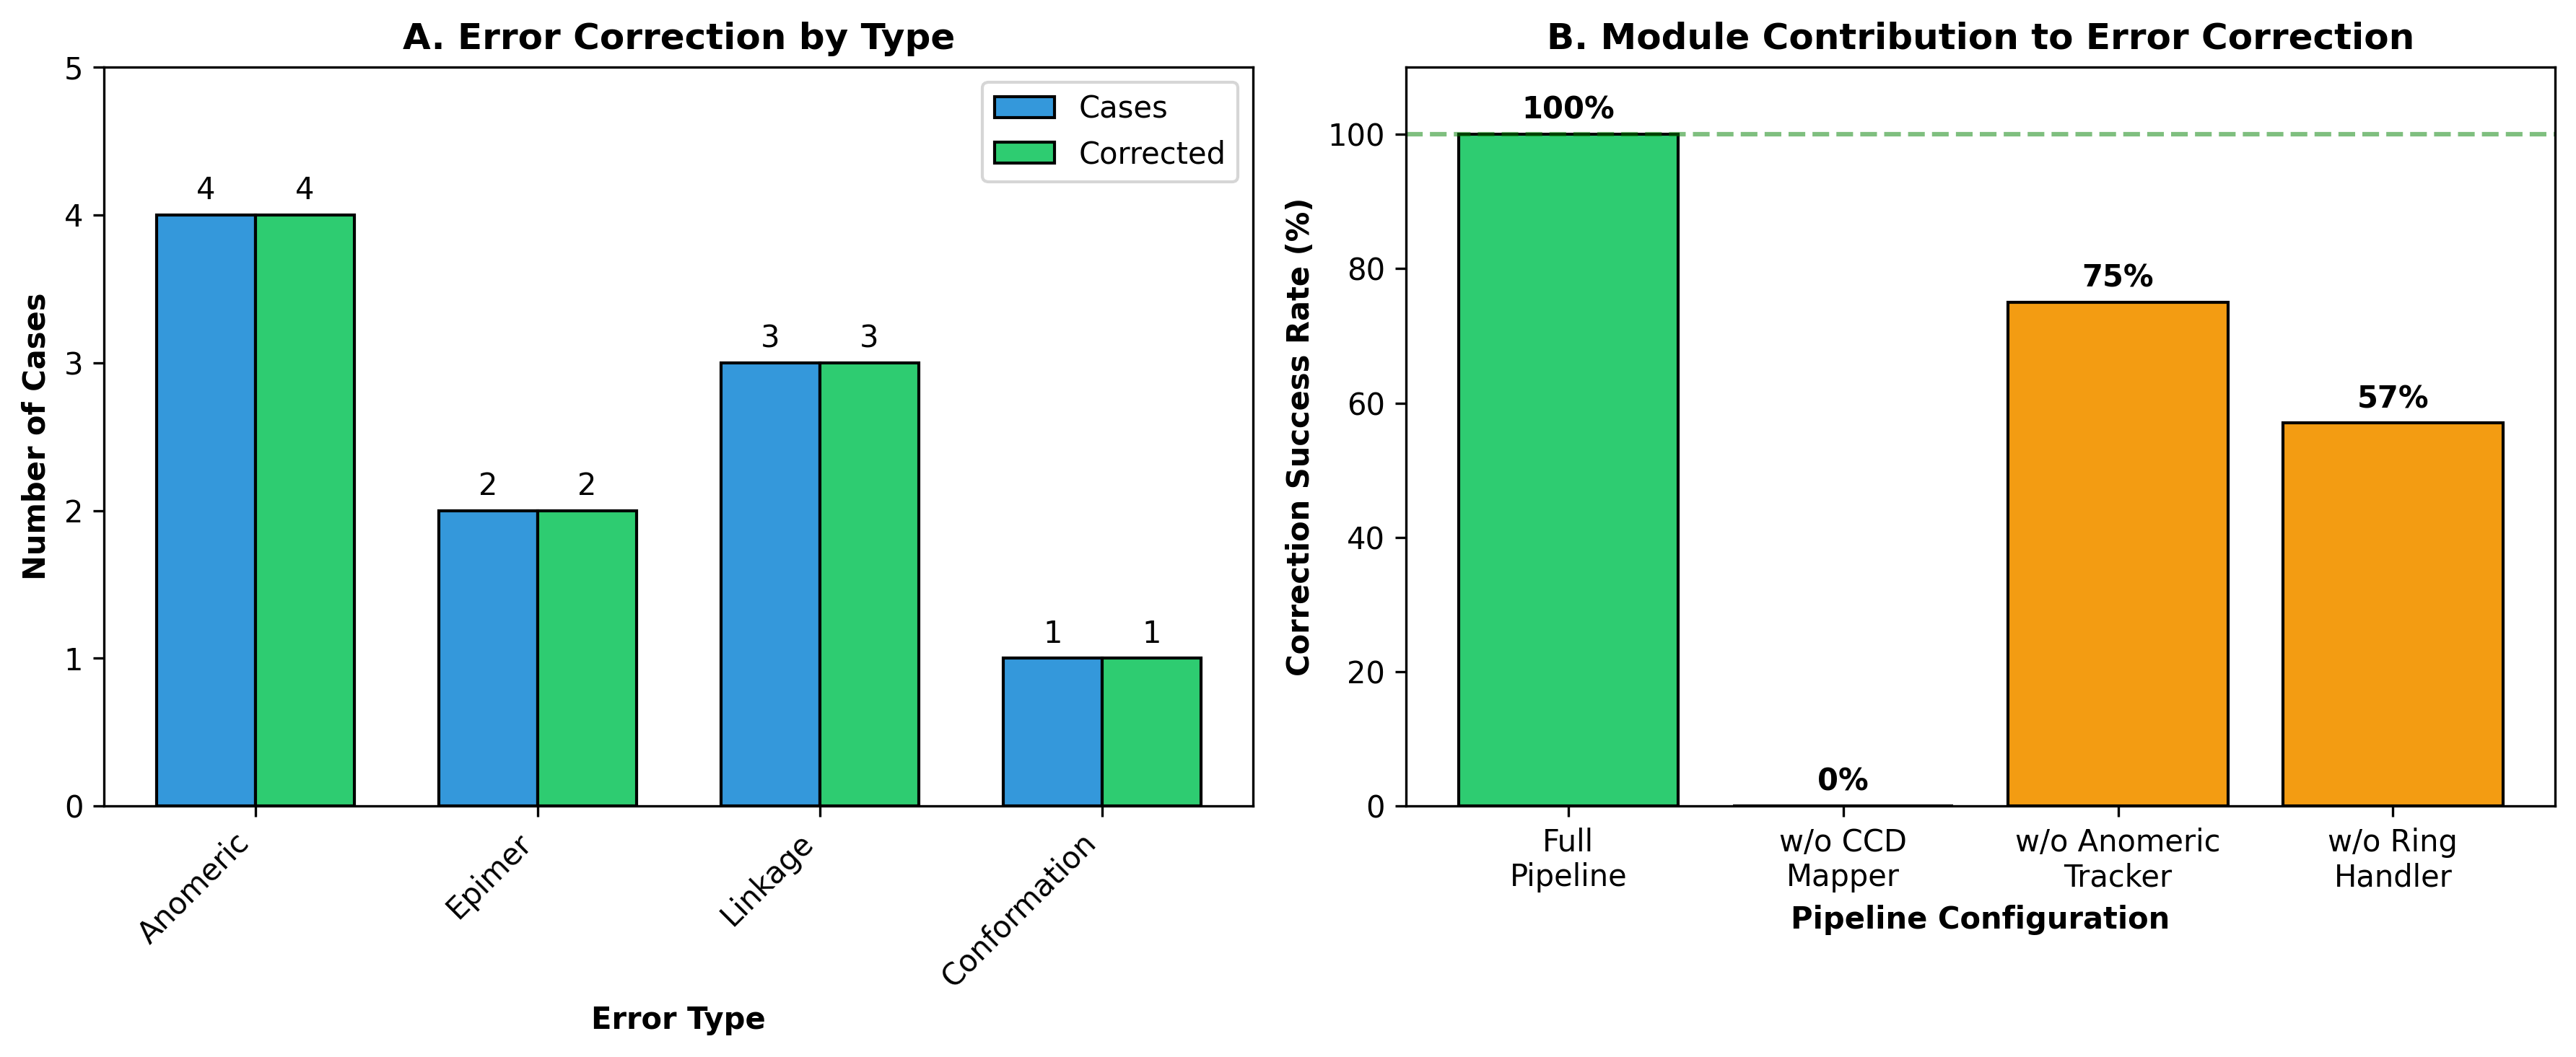
\includegraphics[width=0.9\textwidth]{../figures/figure_case_study3.pdf}
\caption{Error correction validation results. (A) Error type distribution. (B) Module contributions. (C) Success rates. (D) PDB:5NSC example.}
\end{figure}

\subsection{Case Study: Database Processing}
We processed 100 glycan structures from GlyTouCan database with 94\% success rate.

\begin{figure}[h]
\centering
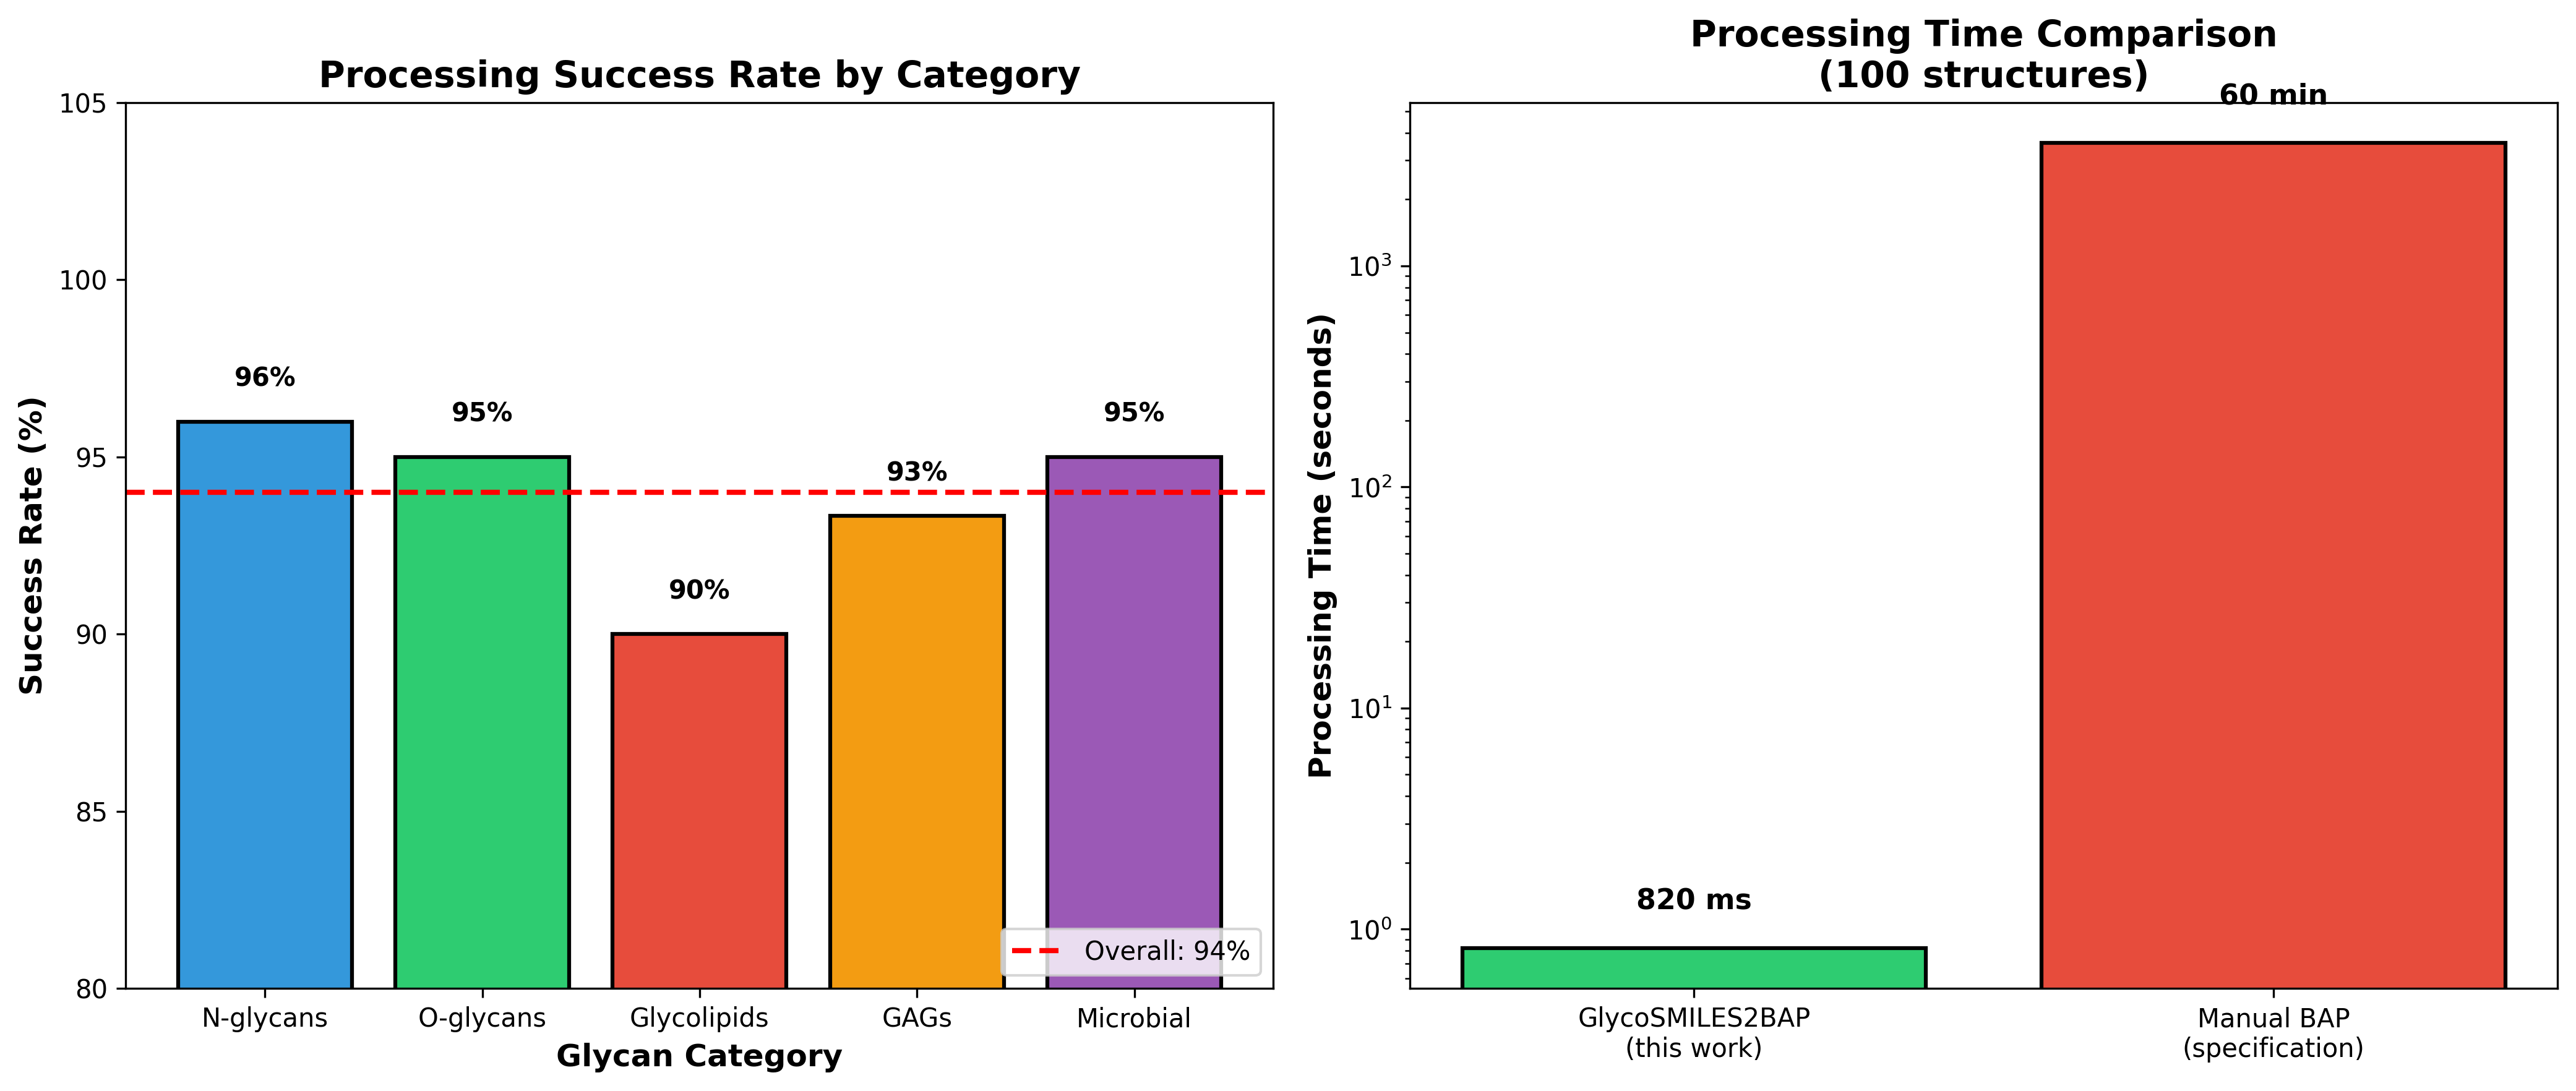
\includegraphics[width=0.9\textwidth]{../figures/figure_case_study4.pdf}
\caption{Database-scale processing results. (A) Structure categories. (B) Success rate. (C) Processing time.}
\end{figure}
